% ================================================================
\section{Sequence Diagrams}

The following diagrams illustrate the main message-passing flows between agents.
Each arrow represents a \texttt{send\_m} or \texttt{messageA} call in the DALI source.

\subsection{Startup Sequence}

\begin{figure}[H]
  \centering
  \includegraphics[width=\textwidth]{../../imgs/01_startup.png}
  \caption{Startup sequence: all agents register with the semaphore, which runs the lights
           sequence and fires \texttt{start\_race} to the first car.}
  \label{fig:seq_startup}
\end{figure}

\subsection{Lap Round-Robin}
\label{sec:round_robin}

\begin{figure}[H]
  \centering
  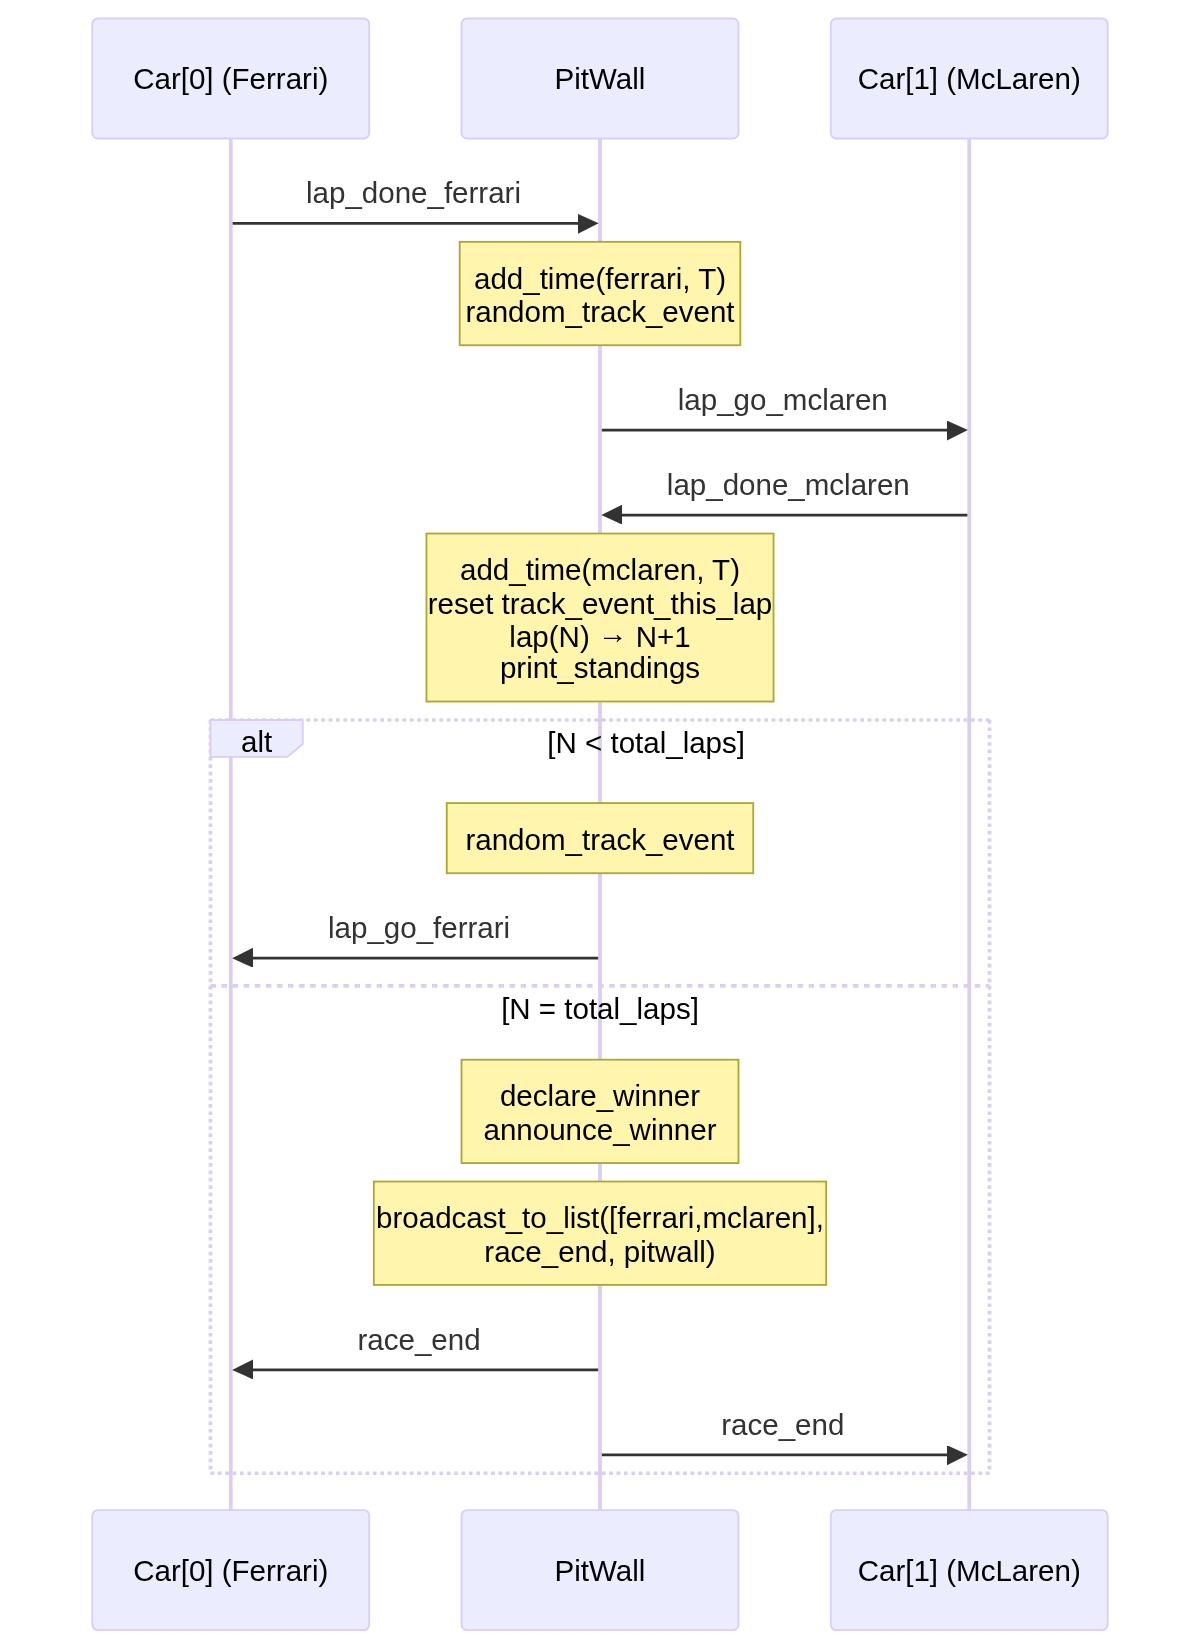
\includegraphics[width=\textwidth]{../../imgs/02_lap_roundrobin.png}
  \caption{Lap round-robin: the pit wall dispatches \texttt{lap\_go} tokens in order,
           accumulates lap times, and increments the lap counter after the last car.}
  \label{fig:seq_lap}
\end{figure}

\subsection{Safety Car Deployment}

\begin{figure}[H]
  \centering
  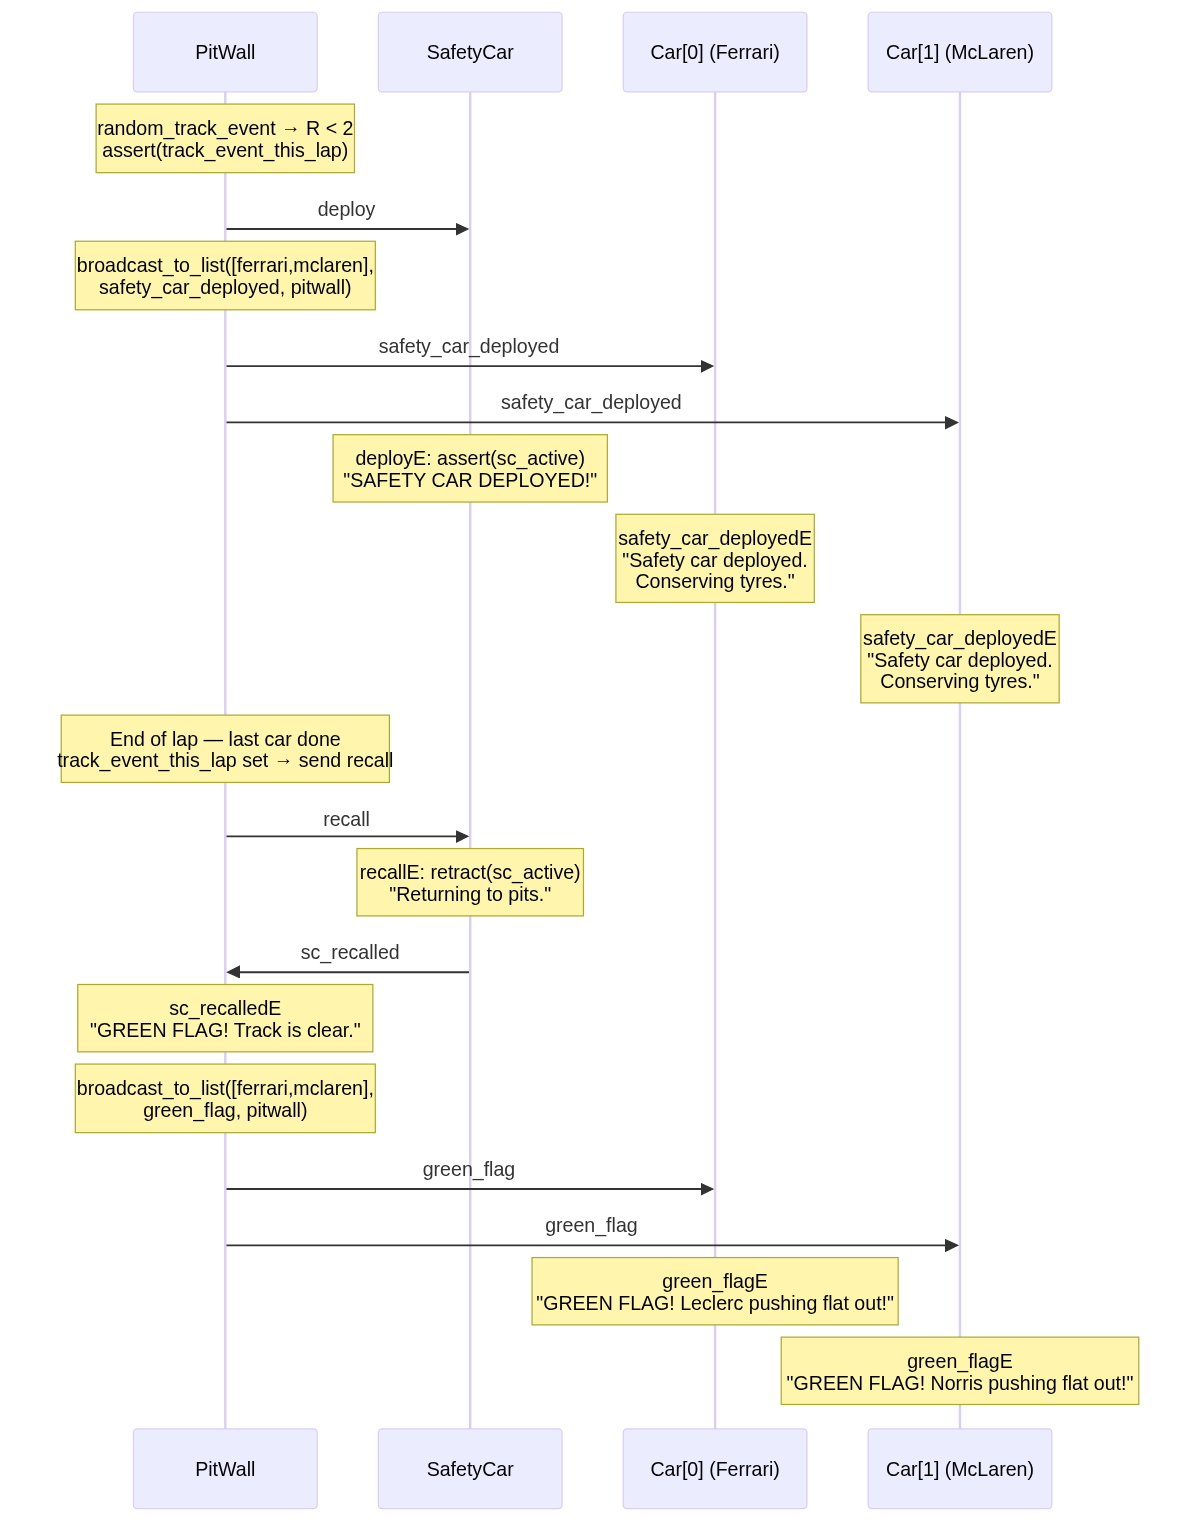
\includegraphics[width=\textwidth]{../../imgs/03_safety_car.png}
  \caption{Safety car chain: pit wall deploys the safety car and notifies all cars;
           at the end of the lap the safety car is recalled and the green flag is broadcast.}
  \label{fig:seq_sc}
\end{figure}

\subsection{Engine Failure (DNF)}

\begin{figure}[H]
  \centering
  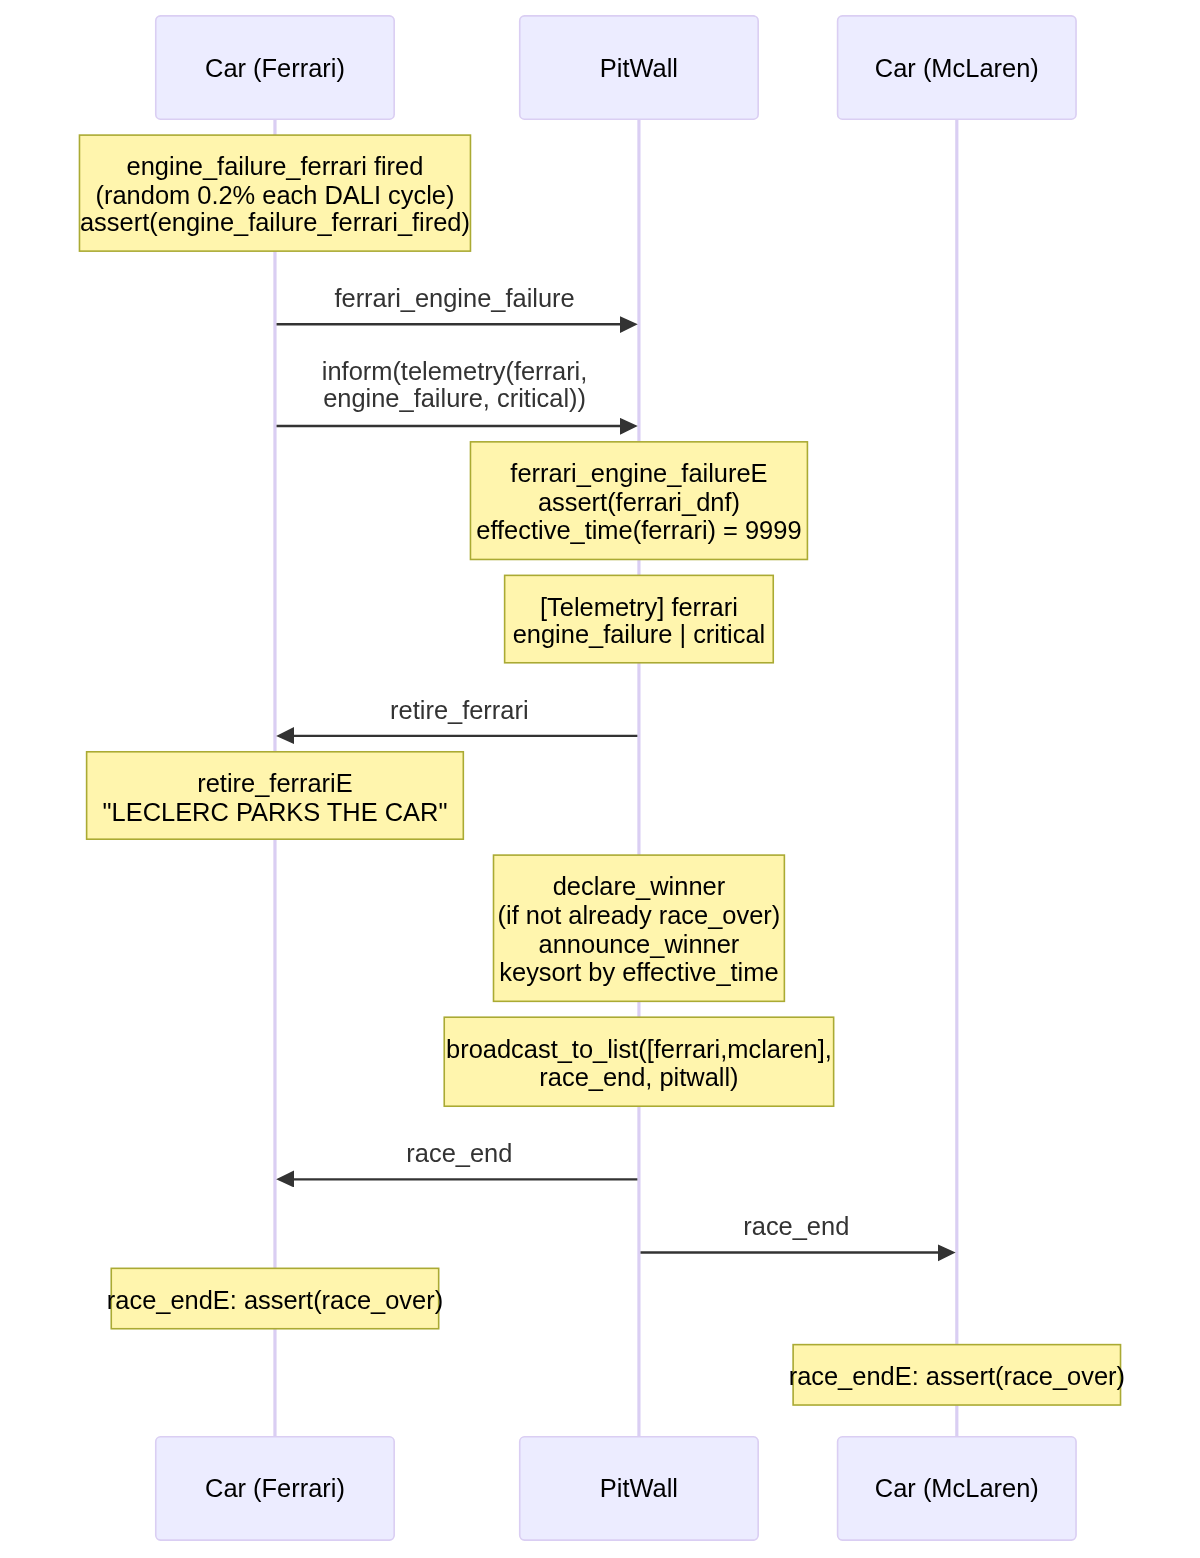
\includegraphics[width=\textwidth]{../../imgs/04_engine_failure.png}
  \caption{Engine failure: a car's internal event notifies the pit wall, which sets the
           DNF time, retires the car, and immediately calls \texttt{declare\_winner}.}
  \label{fig:seq_dnf}
\end{figure}
